\documentclass[10pt]{article}

\usepackage{amsmath}
\usepackage{fullpage}
\usepackage{array}
\usepackage{graphicx}
\usepackage{gensymb}
\usepackage{booktabs}
\usepackage{gensymb}
\usepackage{graphicx}
\usepackage{hyperref}
\hypersetup{colorlinks,urlcolor=blue}
\usepackage{mathtools}


\graphicspath{ {../Images/} }

\date{2014-6-22}
\pagestyle{empty}
\setlength{\parindent}{0pt}

\begin{document}
\begin{center}
\begin{Large}\textbf{Chapter: Work Energy}\end{Large} \\
\smallskip
%\begin{large} Acceleration \end{large}
\end{center}
%%%%%%%
Objectives: Conservative forces, Potential energy (gravitational, spring), Conservation of mechanical energy.
\section{Potential energy}
Earlier in the class we learnt that there is an energy associated with the motion of the object and it is known as kinetic energy.  In the last activity, we discovered that energy can be stored in the spring.  The amount of energy stored in the spring depends on the magnitude of the extension of the spring.  This energy is called potential energy.  For spring the potential energy is given by
\begin{equation}
  PE = \frac{1}{2}kx^2
\end{equation}
where $k$ is called the spring constant.  It follows from the Hooke's law which states that the force/tension developed in the string is \emph{lineraly} proportional to the extension in the spring.  It is given by
\begin{equation}
  F = -kx
\end{equation}
where $k$ is the spring constant and $x$ is the extension in the spring as shown in the figure \ref{springhooke}.
\begin{figure}[h]
\label{springhooke}
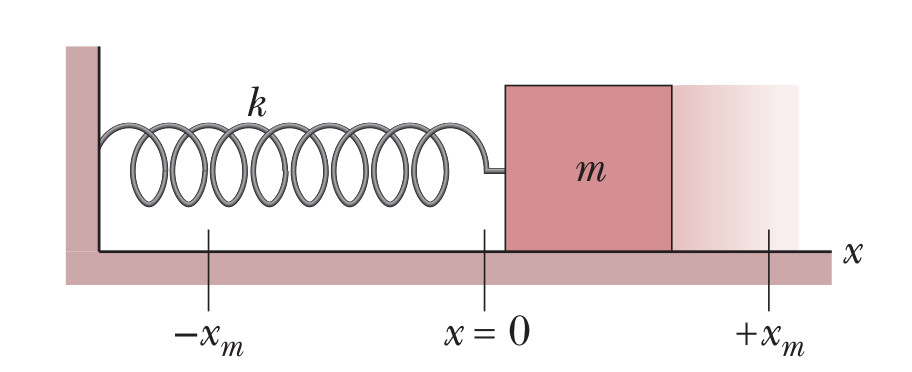
\includegraphics[scale=1]{springhooke}
\centering
\caption{Spring mass system}
\centering
\end{figure}
Note that the direction of the force is \emph{opposite} to that of the extension produced in the spring.

Now the $PE$ of the spring is only dependent on the initial and the final position of the mass (how?).  Such potentials are produced by the forces known as the \emph{conservative forces}.  Gravitational force is another example of a conservative force.  Therefore the potential energy associated with the objects in gravitational field should also depend only on the initial and final position of the mass.  

\begin{figure}[h]
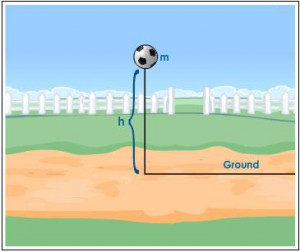
\includegraphics[scale=.5]{potenergyfootball}
\centering
\caption{Football at height $h$}
\label{potfootball}
\centering
\end{figure}
Consider a football tossed up at the height $h$ from the ground as shown in the figure \ref{potfootball}.  Then the potential energy of the football is given by the formula
\begin{equation}
  PE = mgh
\end{equation}
where $m$ is the mass of the football and $g$ is the acceleration due to gravity.
\section{Mechanical Energy}
The mechanical energy of the system is the linear sum of the potential energy and kinetic energy.  Symbolically
\begin{equation}
\begin{split}
  ME &= KE + PE\\
&= \frac{1}{2}mv^2 + \left(\underbrace{mgx}_{\text{Gravity system}}\text{ or }\underbrace{\frac{1}{2}kx^2}_{\text{Spring system}}\right)
\end{split}
\end{equation}
Now the law of the conservation of energy says that the total mechanical energy of the system is conserved in absence of the external force.  Actually this law is a consequence of a very beautiful theorem by \href{https://en.wikipedia.org/wiki/Emmy_Noether}{Emmy Noether} known as \href{https://en.wikipedia.org/wiki/Noether%27s_theorem}{Noether's Theorem}.  I would highly recommend reading the wikipedia page included in the hyperlink. 
\section{Sample Questions}
\begin{enumerate}
\item An athlete runs on the tracks at the speed 9 m/s.  Her mass is 50 kg.  Find the kinetic energy of the athlete on the tracks.  Assuming that the tracks are 100 m long, how much time does it take for the athlete to complete the run?
\item Consider the figure \ref{potfootball}.  The football was tossed up with the speed of 24 m/s.  Assuming that the mass is .5 kg and acceleration due to the gravity is 10 m/s, find the maximum height of the football.  Verify the law of conservation of energy at the bottom most and top most point.
\item In the figure \ref{smassramp}, a block slides along a track that descends through distance $h$.  The track is frictionless except for the lower section.  There the block slides to a stop in a certain distance $D$ because of the friction.
  \begin{enumerate}
  \item If we decrease $h$, will the block now slide to a stop in a distance that is greater than, less than, or equal to $D$?
   \item If, instead, we increase the mass of the block, will the stopping distance now be greater than, less than, or equal to $D$?
  \end{enumerate}
\begin{figure}[h]
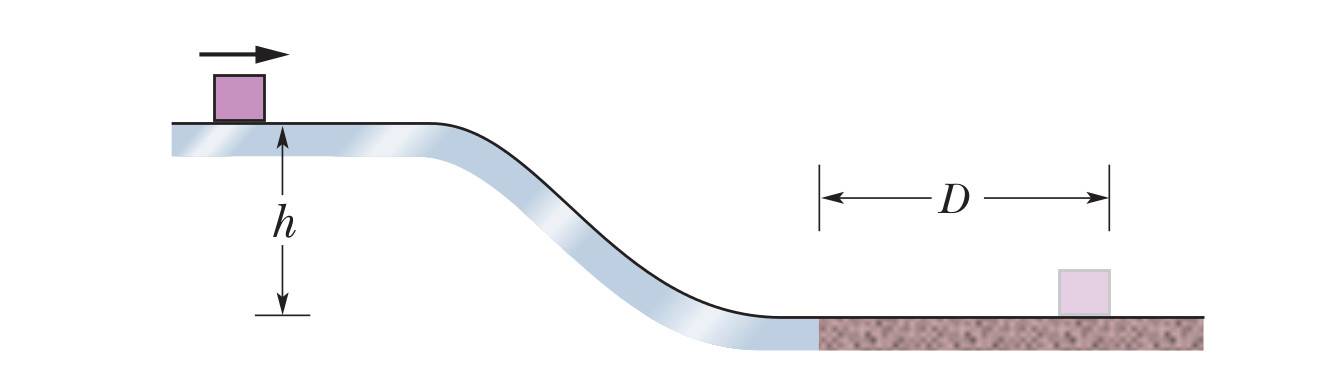
\includegraphics[scale=1]{slidingmasspot}
\centering
\caption{Sliding mass on the ramp}
\label{smassramp}
\centering
\end{figure}
\end{enumerate}
\end{document}
